\iffalse
This is a big-ish template that I've been using for years now.
A lot of the includes are redundant, so if you're reading this and have no idea why
I've included most things, don't worry - I don't either.
Also, compiling this (to PDF, for instance) relies on CSS files present on my
computer (coming from the packages). So it might not look as nice if you
do it on yours (especially if you don't have all the packages).

Ya'll've been warned.
\fi

\documentclass{article}

    \usepackage{tikz}
    \usetikzlibrary{%
        decorations.pathreplacing,%
        decorations.pathmorphing%
    }
    \usepackage{subcaption}
    \usepackage{todonotes}
    \usepackage{amsmath}
    \usepackage{amssymb}
    \usepackage{color}
    \usepackage{bm}
    % \usepackage[dvipsnames]{xcolor}
    \usepackage{graphicx,float}
    \usepackage{caption}
    \usepackage{float}
    \usepackage[hidelinks]{hyperref}
    \usepackage{enumitem}
    \usepackage[bottom]{footmisc}
    \usepackage{flexisym}
    \usepackage{cancel}
    \usepackage[braket]{qcircuit}
    \usepackage[margin=.8in, tmargin=.3in]{geometry}
    \usepackage{mathtools}  %
    \renewcommand{\baselinestretch}{1.2}
    \newcommand{\eps}{\epsilon}


    \newcommand{\vq}{\mathbf{q}}
    \newcommand{\vqdot}{\mathbf{\dot{q}}}
    \newcommand{\vqddot}{\mathbf{\ddot{q}}}
    \newcommand{\vx}{\mathbf{x}}
    \newcommand{\vy}{\mathbf{y}}
    \newcommand{\vystar}{\mathbf{y}^*}
    \newcommand{\vu}{\mathbf{u}}
    \newcommand{\vv}{\mathbf{v}}
    \newcommand{\vf}{\mathbf{f}}
    \newcommand{\vr}{\mathbf{r}}
    \newcommand{\vp}{\mathbf{p}}
    \newcommand{\vg}{\mathbf{G}}
    \newcommand{\bM}{\mathbf{M}}
    \newcommand{\bC}{\mathbf{C}}
    \renewcommand{\vec}{\bm}
    \newcommand{\dotvec}[1]{\bm{\dot{#1}}}
    \newcommand{\bS}{\mathbf{S}}
    \newcommand{\bJ}{\mathbf{J}}
    \newcommand{\vlam}{\pmb{\lambda}}
    \newcommand{\vxdot}{\mathbf{\dot{x}}}
    \newcommand{\argmin}{\operatornamewithlimits{arg\ min}}

    % \newcommand{\tens}{\otimes}


\newcommand{\tens}[1]{%
  \mathbin{\mathop{\otimes}\limits_{#1}}%
}

    \setlength{\parskip}{\baselineskip}
    % \newcommand{\l}{\left(}
    
    \usepackage{titlesec}
    \usepackage{physics}
    \usepackage{multicol}
    
    \setlength\parindent{0pt}
    \captionsetup{justification=centering}
    
    \title{Classical Mechanics: From Newton to Euler-Lagrange}
    \date{\today}
    \author{Traiko Dinev \textless traiko.dinev@gmail.com\textgreater}

\begin{document}
\begin{multicols}{2}[Classical Mechanics: From Newton to Euler-Lagrang]
\maketitle
\textit{NOTE: These notes are a summary of Classical Mechanics: A Theoretical Minimum. They also contain some of David Morrin. Some of the notebooks are exercises I did through my own research.}

\textit{NOTE: Note this "summary" is NOT a reproduction of the course materials nor is it copied from the corresponding courses. It was entirely written and typeset from scratch.}

\textit{License: Creative Commons public license; See README.md of repository}

Hey, it is me, the author of these notes. I used to think reading physics was pointless practically speaking, so I did it a bit sparingly. But then.. I actually needed it in my own research! So I'm citing my work here~\cite{dinev2020modeling}. Hopefully it encourages more academics to read physics at a moderate to advanced level, as you never know when you'll need it!


\section{Basics}
A position of a particle in space is $\bm{r} = (x, y, z)$, its velocity is $\bm{v} = \dot{\bm{r}} = \frac{d\bm{r}}{d t}$. By (almost) definition of derivatives, we have:

\begin{equation}
    \bm{r}(t) = \bm{r}_0 + \bm{v}_0 t
\end{equation}

if $\bm{v}(t) = \bm{v}_0$ is independent of time. Adding acceleration to this, by \textbf{Newton's second law}, $\bm{a} = \dot{\bm{v}} = \bm{F}/m$, we can arrive at the following differential equation:

\begin{equation}
    \dot{\bm{r}}_t = \bm{v}(t) = \bm{v}_0 + \bm{a}_0 t
\end{equation}

Integrating this, we obtain:

\begin{align}
    \bm{r}(t) &= \bm{r}_0 + \int_0^t \bm{v}(t) dt = \bm{r}_0 +  \int_0^t \bm{v}_0 + \bm{a}_0 t\ dt \\
    &= \bm{r}_0 + \bm{v}_0 t + \frac{\bm{a}_0}{2} t^2 = \bm{r}_0 +  \bm{v}_0 t + \frac{\bm{F}}{2m} t^2
\end{align}

assuming that the acceleration is not a function of time. Otherwise you'd integrate the above ODE for each timestep.

\section{Generalized Co-ordinates and Equations of Motion}
\textit{The following is from a robotics summary of mine}

    A system's dynamics are most generally described by a second-order non-linear equation:

    \begin{equation} \label{eq:dynamics}
        \ddot{\vec{q}} = \vec{f}(\vec{q}, \dot{\vec{q}}, \vec{u}, t)
    \end{equation}

    where $\dot{\vec{q}}$ and $\ddot{\vec{q}}$ are the first and second derivative of $\vec{q}(t)$ -- the state of the system and $\vec{u}(t)$ -- the control inputs at time $t$. $\vec{f}$ is a matrix describing the dynamics. \autoref{eq:dynamics} describes the time-evolution of the world's configuration. This depends on the state at time $t$ as well as the control inputs we apply. We derive the equations of motion by using Newton's second law of motion. For all robots without kinematic chains (loop mechanical connections), the above can be generally written as the following product:

    \begin{equation} \label{eq:dynamics_standard}
        \vec{M}(\vec{q}) \ddot{\vec{q}} + \vec{C}(\vec{q}, \dot{\vec{q}}) \dot{\vec{q}} =
            \tau_g(\vec{q}) + \vec{B}\vec{u}
    \end{equation}

    Here $\vec{M}$ is the inertia matrix, $\vec{C}$ is the Coriolis matrix, $\tau_g$ is the gravity vector and $\vec{B}$ maps control inputs $\vec{u}$ into forces. For many systems this simplifies even further:

    \begin{equation} \label{eq:affine}
        \ddot{\vec{q}} = \vec{f}_1(\vec{q}, \dotvec{q}, t) + \vec{f}_2(\vec{q}, \dotvec{q}, t)\ \vec{u}
    \end{equation}

    We call such systems \textbf{control affine}. Such systems have dynamics that are affine (linear plus offset) in $\vec{u}$.

\section{Lagrange}
So how do we obtain the equations of motion of a system? They all obey Newton's second law, but there is another way of stating that is more general. Define the Lagrangian of a system as the difference of its kinetic energy and potential energy:

\begin{equation*}
    \mathcal{L} = T - V
\end{equation*}

The fundamental law then states that for any system the motion from point A to point B is that which minimizes the integral of this difference along the path. In a sence it is a \textbf{stationary action principle}, that is the action (the integral) is stationary (not necessarily a minimum or maximum). Firstly, let's start with conservative forces (which as we'll see will make a certain term equal to 0). We write the integral of the lagrangian as:

\begin{equation*}
    S = \int_{t_A}^{t_B} \mathcal{L}\ dt
\end{equation*}

and we call $S$ the \textbf{action}. The principle states that the action is stationary, i.e.:

\begin{equation*}
    \delta S = 0
\end{equation*}

In generalized coordinates the system's kinetic energy is $\frac{1}{2} \dot{q}^T M \dot{q}$. For readability we will stick to the one-dimensional case, trusting that this extends (and it does) to any dimensions. For now, all we need to know is that the Lagrangian $\mathcal{L}$ is a function of time, generalized positions, and generalized velocities:

\begin{equation*}
    \mathcal{A} = \mathcal{A}(t, q(t), \dot{q}(t))
\end{equation*}

Firstly, we need to be clear that the path a system takes must start and end at a fixed point (otherwise this doesn't work), that is $q(t_A) = q_A, q(t_B) = q_B$ and the same for velocities. We want to find the minimum of the action, that is:

\begin{equation*}
    \min_{q(t)} S = \min \int_{t_A}^{t_B} \mathcal{L}\ dt
\end{equation*}

where we note two things. 1) we are minimizing w.r.t. a function and 2) -- we are minimizing an integral.
Consider a petrubation of the path the system takes (the thing under the min above):

\begin{align*}
    q'(t) &= q(t) + \epsilon \eta(t) \\
    \dot{q}'(t) &= \dot{q}(t) + \epsilon \eta'(t)
\end{align*}

where we need to have $\eta(t_A) = \eta(t_B) = 0$, because we've fixed the start and end points. At the minimum any variation must yield a greater action (flip for maximum), that is:

\begin{equation*}
    S[t, q(t), \dot{q}(t)] \leq S[t, q(t) + \epsilon \eta(t), \dot{q}(t) + \epsilon \eta'(t)]
\end{equation*}

which means that the minimum is at $\epsilon = 0$. Minimum means that the derivative needs to be $0$. First we define the thing that's at the minimum to be a function of $\epsilon$:

\begin{equation*}
    f(\epsilon) = S[t, q'(t), \dot{q}'(t)]
\end{equation*}

Now we can say that this is minimized at $\epsilon = 0$ (follows from the assumption that action is minimized). Then we calculate its total derivative:

\begin{equation}
    \frac{d f}{d \epsilon} = \frac{d}{d \epsilon}\int_{t_A}^{t_B} \mathcal{L}(t, q'(t), \dot{q}'(t))\ dt = \int_{t_A}^{t_B} \frac{d \mathcal{L}}{d \epsilon}\ dt
\end{equation}

The derivative of the Lagrangian w.r.t $\epsilon$ is:

\begin{equation*}
    \frac{d \mathcal{L}}{d \epsilon} = \frac{\partial \mathcal{L}}{\partial t} \frac{d t}{d \epsilon} + \frac{\partial \mathcal{L}}{\partial q'} \frac{dq'}{d \epsilon} + \frac{\partial \mathcal{L}}{\partial \dot{q}'} \frac{d \dot{q}'}{d \epsilon}
\end{equation*}

The first term is $0$ since $\epsilon$ has no effect on $t$. We can do a substitution of the pertrubation derivatives to obtain:

\begin{equation*}
    \frac{d \mathcal{L}}{d \epsilon} = \frac{\partial \mathcal{L}}{\partial q'} \eta(t) + \frac{\partial \mathcal{L}}{\partial \dot{q}'} \eta'(t)
\end{equation*}

note the slighly confusing notation, where $q'$ stands for variation in $q$ and $\eta'$ stands for $\eta$'s derivative. At least we consistenly use the inconsistency. Now the derivative of $f(\epsilon)$ needs to be $0$ at $\epsilon = 0$. This means we can remove all the pertrubations in the Lagrangian (set $q' = q, \dot{q}' = \dot{q}$) Meaning:

\begin{equation*}
    \left. \frac{d \mathcal{L}}{d \epsilon} \right\vert_{\epsilon = 0} = \int_{t_A}^{t_B} \left[ \frac{\partial \mathcal{L}}{\partial q} \eta(t) + \frac{\partial \mathcal{L}}{\partial \dot{q}} \eta'(t) \right] dt = 0
\end{equation*}

Next we need to integrate by parts. Remembering that if we have:

\begin{equation*}
    \frac{d\ \eta f}{dt} = \eta \frac{df}{dt} + f \frac{d\eta}{dt}
\end{equation*}

then we can integrate to get:

\begin{equation*}
    \int f \frac{d \eta}{dt} dt = \eta f - \int \eta \frac{df}{dt} dt
\end{equation*}

We apply integration by parts on the second term:

\begin{align*}
    & \int_{t_A}^{t_B} \left[ \frac{\partial \mathcal{L}}{\partial q} \eta(t) + \frac{\partial \mathcal{L}}{\partial \dot{q}} \eta'(t) \right] dt \\
    & = \int_{t_A}^{t_B} \frac{\partial \mathcal{L}}{\partial q} \eta(t)\ dt +
        \int_{t_A}^{t_B} \frac{\partial \mathcal{L}}{\partial \dot{q}} \eta'(t) dt \\
    & = \int_{t_A}^{t_B} \frac{\partial \mathcal{L}}{\partial q} \eta(t)\ dt + 
        \left[ \frac{\partial \mathcal{L}}{\partial\dot{q}} \eta(t) \right]_{t_A}^{t_B}
        - \int_{t_A}^{t_B} \frac{d}{dt} \frac{\partial \mathcal{L}}{\partial \dot{q}} \eta(t) \ dt \\
    & = \int_{t_A}^{t_B} \frac{\partial \mathcal{L}}{\partial q} \eta(t)\ dt
    - \int_{t_A}^{t_B}  \frac{d}{dt} \frac{\partial \mathcal{L}}{\partial \dot{q}} \eta(t)\ dt \\
    & = \int_{t_A}^{t_B} \left[ \frac{\partial \mathcal{L}}{dq} \eta(t) - \frac{d}{dt} \frac{\partial \mathcal{L}}{\partial \dot{q}} \eta(t) \right] \ dt = \\
    & = \int_{t_A}^{t_B} \left[ \frac{\partial \mathcal{L}}{\partial q} - \frac{d}{dt} \frac{\partial \mathcal{L}}{\partial\dot{q}} \right] \eta(t) \ dt
\end{align*}

where we apply the bundary conditions $\eta(t_A) = \eta(t_B) = 0$. Now we have this remaining:

\begin{equation*}
    \int_{t_A}^{t_B} \left[ \frac{\partial \mathcal{L}}{\partial q} - \frac{d}{dt} \frac{\partial \mathcal{L}}{\partial \dot{q}} \right] \eta(t) \ dt = 0
\end{equation*}

where this is true at $\epsilon = 0$. Feynman has the best visual proof but the idea is that if it's true for any $\eta(t)$ I can make it any delta function (peak) $\eta(t_i) =  1$ for any $i$ I choose then the first thing must be 0. Meaning:

\begin{equation}
    \frac{\partial \mathcal{L}}{\partial q} - \frac{d}{dt} \frac{\partial \mathcal{L}}{\partial \dot{q}} = 0
\end{equation}

Normally this is written the other way around:

\begin{equation}
    \frac{d}{dt} \frac{\partial \mathcal{L}}{\partial \dot{q}} - \frac{\partial \mathcal{L}}{\partial q} = 0
\end{equation}

The conservative forces show as potential energies. Namely:

\begin{align*}
    \mathcal{L} &= T - V \\
    T &= \frac{1}{2} m \dot{q}^2 \\
    F_{pot} &= -\frac{d V}{dt}
\end{align*}

with a negative sign convention in physics. This is just Newton's second law for a particle:

\begin{align*}
    \mathcal{L} &= \frac{1}{2} m v^2 - V(x) \\
    \frac{d}{dt} m v&= -\frac{d V(x)}{dt} \\
    m a &= F
\end{align*}


Lastly, remember external (non-conservative) forces? They show up on the right:

\begin{equation}
    \frac{d}{dt} \frac{\partial \mathcal{L}}{\partial \dot{q}} - \frac{\partial \mathcal{L}}{\partial q} = F_{ext}
\end{equation}

\section{Example}

\begin{figure}[H]
    \centering
    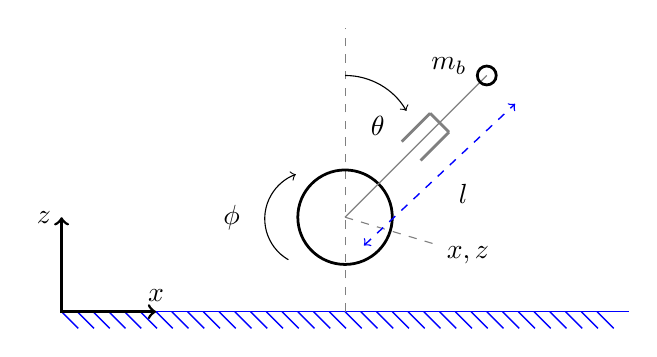
\begin{tikzpicture}[
        media/.style={font={\footnotesize\sffamily}},
        interface/.style={
            postaction={draw,decorate,decoration={border,angle=-45,
                        amplitude=0.3cm,segment length=2mm}}},
        scale=1.2
        ]
        
        % Round rectangle
        % \fill[gray!10,rounded corners] (-4,-3) rectangle (4,0);
        % Interface
        \draw[blue,line width=.5pt,interface](-3,0)--(3,0);
        % Vertical dashed line
        \draw[dashed,gray](0,0)--(0,3);


        % Coordinates system
        % \draw(0,0.15)node[above]{$x$};
        \draw[<->,line width=1pt, shift={(-3cm, 0cm)}] (1,0) node[above]{$x$}-|(0,1) node[left]{$z$};


        \path (0,0)++(80:2.cm)node{$\theta$};
        \draw[->] (0,2.5) arc (90:30:.75cm);


        \path (0,0)++(-1.2, 1)node{$\phi$};
        \draw[->] (-.6,.55) arc (-120:-250:.5cm);

        \draw[gray,dashed](0,1)--(1,.7);
        \path (1.3, .6)node{$x,z$};



        \draw[line width=1pt](0,1cm)circle(.5cm);
        \draw[gray](0,1)--(1.5,2.5);

        \draw[gray, line width=1pt](1.1, 1.9)--(0.9,2.1);
        \draw[gray, line width=1pt](0.9,2.1)--(0.6,1.8);
        \draw[gray, line width=1pt](1.1,1.9)--(0.8,1.6);

        \draw[line width=1pt](1.5,2.5)circle(.1cm);
        \path(1.1, 2.6) node{$m_b$};


        \draw[<->,line width=.5pt,blue,dashed](0.2,0.7)--(1.8, 2.2);
        \path (1.25, 1.25) node{$l$};
    \end{tikzpicture}

    \caption{A Variable-Length Wheeled Inverted Pendulum (VL-WIP) model.}
    \label{fig:dynamics}
\end{figure}


We use the Lagrangian method to derive the dynamics of the system.
First, we define the position $x_b, z_b$ of the mass $m_b$ and its velocity $\dot{x}_b, \dot{z}_b$:
% 
% \vskip 0.1in
\begin{align}
    x_b &= x + l\ \sin(\theta) \\
    z_b &= z + l\ \cos(\theta) \nonumber \\
    \dot{x}_b &= \dot{x} + \dot{l}\ \sin(\theta) +
        l\ cos(\theta)\ \dot{\theta} \nonumber \\
    \dot{z}_b &= \dot{z} + \dot{l}\ \cos(\theta) -
        l\ sin(\theta)\ \dot{\theta} \nonumber
\end{align}
% \vskip 0.1in
% 
Lagrange's method states that for a system with total kinetic energy $T$ and potential energy $U$:
% 
\vskip 0.1in
\begin{equation} \label{eq:lagrange}
    \frac{d}{dt} \frac{\partial \mathcal{L}}{\partial \vqdot_i} - \frac{\partial \mathcal{L}}{\partial \vq_i} = \vf_{ext},
\end{equation}
\vskip 0.1in
% 
where $\mathcal{L} = T - U$ is the system's Lagrangian and $\vf_{ext}$ are external forces applied to the system. We now need to compute the system's kinetic and potential energy.

In general, every link will have a rotational and translational kinetic energy component. For the wheel we include a rotational kinetic energy term $I_w \dot{\phi}^2$ where $I_w = m_w R_w^2$ is the moment of inertia of the wheel. Since the point mass has a zero moment of inertia, it only has a translational kinetic energy $m_b \vv_b^T \vv_b$, where $\vv_b$ is the velocity of the point mass.

The only potential energy component is due to gravity $g$ acting on the wheel and the point mass. This leads to:
% 
\begin{align} \label{eq:energy1}
    T &= \frac{1}{2}(I_w \ \dot{\phi}^2 + m_w \dot{x}^2 +
        m_w \dot{z}^2 + m_b \dot{x}_b^2 + m_b \dot{z}_b^2) \\
    U &= m_w g z + m_b g z_b \label{eq:energy2} \\
    \mathcal{L} &= T - U \label{eq:energy3}
\end{align}

\textit{Note} I haven't written it out here, but you will obtain a system of equations, which you can solve however you want (scipy has a package to check your working). Then you can obtain the mass matrix, the coriolis matrix and the gravity vector.


\section{Conservation Laws (Noether)}
\subsection{Generic Proof (Simplified)}
A symmetry is defined as $\delta S = 0$ for a certain variation in the path. As before, we define:

\begin{align*}
    q_i'(t) &= q_i(t) + \eta_i(q(t), t) \\
    \delta q_i &= q_i'(t) - q_i(t) = \eta_i(q(t), t)
\end{align*}

for all the generalized coordinates $q_i$. Then, since the action is invariant under the symmetry, we have:

\begin{equation*}
    \delta S = S[q'] - S[q] = 0
\end{equation*}

Noether's theorem states that the quantity (Q):

\begin{equation*}
    Q = \sum_i \frac{\partial \mathcal{L}}{\partial \dot{q}_i} \eta_i
\end{equation*}

Starting with the action vanishing, we have:

\begin{align*}
    &\delta S = \sum_i \int_{t_A}^{t_B} \delta \mathcal{L}\ dt
         = \int_{t_A}^{t_B} \frac{\partial \mathcal{L}}{\partial q_i} \delta q_i + \frac{\partial \mathcal{L}}{\partial \dot{q}_i} \delta \dot{q}_i\ dt = \\
    &= \sum_i \int_{t_A}^{t_B} \frac{\partial \mathcal{L}}{\partial q_i} \eta_i + \frac{\partial \mathcal{L}}{\partial \dot{q}_i} \eta'_i \ dt = \\
    &= \sum_i \int_{t_A}^{t_B} \left[ \frac{d}{dt} \frac{\partial \mathcal{L}}{\partial \dot{q}_i} - \frac{\partial \mathcal{L}}{\partial q_i} \right] \eta_i\ dt - \left. \frac{\partial \mathcal{L}}{\partial \dot{q}_i} \eta_i \right\vert_{t_A}^{t_B}
\end{align*}

where we used the same integration by parts trick as before. Now, if the system obeys the Newton-Euler equation of motion, then the integral vanishes and we have:

\begin{align*}
    \delta S = \sum_i \left. \frac{\partial \mathcal{L}}{\partial \dot{q}_i} \eta_i \right\vert_{t_A}^{t_B} = Q(t_B) - Q(t_A) = 0
\end{align*}

Since we did not specify or impose any constraints on $t_A$ and $t_B$, this is valid for any path. Thus:

\begin{align*}
    \frac{d}{dt} \sum_i \frac{\partial \mathcal{L}}{\partial \dot{q}_i} \eta_i = 0
\end{align*}

and $Q$ is conserved as its derivative is $0$ everywhere along the path.


\subsection{Back to Physics}
First we need a couple of definitions. A \textbf{cyclic coordinate} is one that does not occur in the Lagrangian, i.e.:

\begin{equation}
    \frac{\partial \mathcal{L}}{\partial q} = 0
\end{equation}

The \textbf{conjugate momemtum} is defined as:

\begin{equation}
    p = \frac{\partial \mathcal{L}}{\partial \dot{q}}
\end{equation}


\subsubsection{Translational Invariance Leads to Conservation of Linear Momentum}
Consider a translation transformation:

\begin{equation*}
    q_i' = q_i + \epsilon_i
\end{equation*}

Then if the Lagrangian is invariant under such a transformation, the quantinity:

\begin{equation*}
    Q = \sum_i \frac{\partial \mathcal{L}}{\partial \dot{q}_i} \epsilon_i
\end{equation*}

is conserved and so is the conjugate momentum, since $\epsilon$ is a constant.

\subsubsection{Total Linear Momentum Conservation}
Consider a vector potential that only depends on the relative distance between $N$ particles $\bm{x}_i$, where $i \in [1, N]$:

\begin{equation*}
    \mathcal{L} = \sum_i \left[ m_i \frac{1}{2} \dot{\bm{x}}_i^T \dot{\bm{x}}_i - \sum_{b \neq a} V(\bm{x}_a - \bm{x}_b) \right] 
\end{equation*}

Then shifting the entire system by the same vector does not change the lagrangian and the action. The velocity change is $0$ and the potential change is also $0$ as:

\begin{align*}
    \bm{x}_i' &= \bm{x}_i + \bm{\epsilon} \\
    \bm{x}_a' - \bm{x}_b' &= (\bm{x}_a + \bm{\epsilon}) - (\bm{x}_b + \bm{\epsilon}) = \bm{x}_a - \bm{x}_b
\end{align*}

which means that:

\begin{equation*}
    Q = \sum_i \frac{\partial L}{\partial \dot{\bm{x}}_i} = 
        \sum_i m_i \bm{\dot{x}}_i
\end{equation*}

is conserved. This is the sum linear momentum of the system.

\subsubsection{Rotational Invariance Leads to Angular Momentum Conservation}
TODO

\section{Time-Translational Invariance Leads to Energy Convervation}

\section{Harmonic Oscillator: Hamiltonians}

\section{Gibbs Liouville}

\section{Poisson Brackets}

\section{Electromagnetic Force}
\subsection{Lorentz Force Law}
\subsection{Vector Potential}
\subsection{Gauge Invariance}

\bibliographystyle{IEEEtran}
\bibliography{IEEEabrv,IEEEconf,bib}
\end{multicols}
\end{document}
